\chapter{\label{ranking-algorithms}Ranking algorithms}

The main purpose of the algorithms discussed below in this section is to answer the question \emph{Given a score, what is the rank of a user or item with this score?}\footnote{\hhref{http://googleappengine.blogspot.se/2009/01/google-code-jams-ranking-library.html}}. The opposite question -- \emph{Given a rank, what is the score for this rank?} is very similar but not adressed here even though most approaches to the ranking problem indirectly answers that question too.

Ranking algorithms can coarsely be divided in two categories: \emph{exact} and \emph{approximating} algorithms. The exact algorithms deal with the ranking problem by sorting and counting the number of users having a better score than the new score. If it is not neccessary to obtain an exact rank or other factors such as speed or cost have to be considered an approximating algorithm can be a good compromise.

Approximating algorithms estimate the rank by interpolation within a segement of ranks. Suitable segments can be found with an \emph{offline-method} such as scanning all scores periodically, keeping track of scores at the segments boundaries (See section \ref{bucket}) or with an \emph{online-method} with a \emph{streaming algorithm} that maintains a model for estimating ranks by continuosly updating a number of statistical measures.

\section{\label{counting}Rank by counting}

The naive approach to ranking a highscore is to count the number of highscores better than the one at hand. This way of getting the rank can be done with a simple query in SQL
\texttt{SELECT count(id) FROM Highscores WHERE Score > TheScore} or by increasing a counter while iterating through an ordered set of highscores in case a non-relational database is used. In any case the items should be indexed on the highscore-field.

Obtaining rank for a score by this method implies scanning through all items having a score higher than the one you want to obtain the rank for. The time complexity of this approach is obviously $\mathcal{O}(n)$ making it unusable for online applications in terms of cost and response time.

\section{\label{sec:tree}Tree based approach}

One way to accomplish counting more efficiently is by storing the count of each score in an N-ary tree. \emph{N} is the maximum number of childrens a node can have. Each node defines $N$ score ranges or $N$ single scores along with their associated count. The leaves represents individual items from the domain of possible scores. The rank for a score is obtained by summing the number of better scores and adding one. An example is provided in Figure \ref{fig:tree}. Updating a score by this approach also implies updating the count in each node visited.

The time complexity of finding a rank in the tree is $\mathcal{O}(\log{} n)$ where $n$ is the number of possible scores. The height of the tree is $\lceil log_{N}n \rceil$. Reading or writing a node may be expensive in case it has to be read from or written to a database system, hence the number of ranges per node needs to be chosen so that the height of the tree remains reasonably low. What would be considered as \emph{reasonably low} depends on details of the implementation such as the cost for database operations, the cost for CPU-time etc. 

There are a number of things to consider with this approach. First, to get exact rankings the leaf nodes will be as many as there are distinct scores. This may be a problem if the range of scores is open in one or both directions. One way to get around that problem could be to not store the count of individual scores but instead count of ranges. This could be done in at least two ways; by defining the ranges in beforehand or by compressing the tree at some interval so that if a childs' score range has only a small number of scores, then do not build the tree further down from that child. That is essentially the solution proposed by Shrivastava et al\cite{quantile_digest} with their Quantile Digest algorithm. A ranking algortihm based on that solution would then not be able to give exact ranks for scores, but have to do approximations. Secondly, if the scores distribution is not known in beforehand the tree may need to be balanced during it's lifetime in order for this class of alghorithms to be efficient.

\begin{figure}[h!]
  \centering
  \caption{Example of how ranking is done using a tree-based approach. To get the rank for score 30, start by adding the counts for scores greater than 30. There is 22 higher scores and rank for score 30 is thus 23.\\This figure is a reproduction of a similar image from the article \emph{Fast and Reliable Ranking in Datastore} \cite{ranking-in-datastore}, licensed under the Creative Commons Attribution 3.0 License}   \label{fig:tree}
\hbox{\hspace{-0.8cm}
  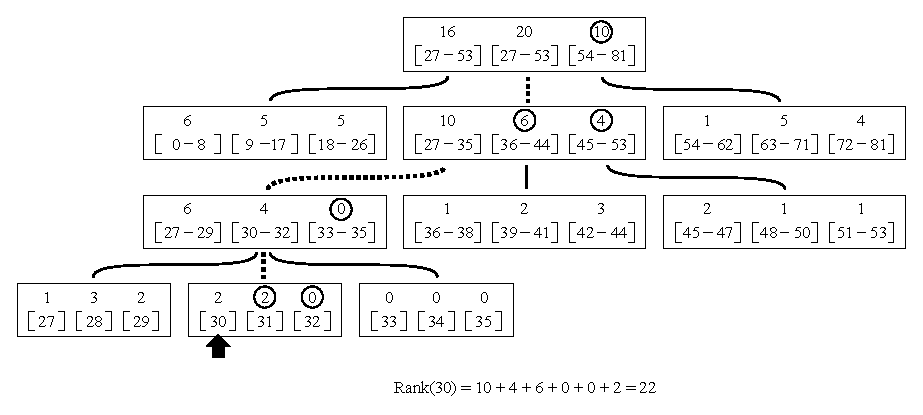
\includegraphics[width=15cm]{img/tree.eps}}
\end{figure}

\section{Rank by approximation with linear interpolation}

Getting an exakt rank for a score may not be crucial. One class of solutions is the ones using linear interpolation to get an approximate rank from a score range and known ranks at the lowest and highest scores. The ranks and score ranges needed for the interpolation can be acquired in different ways of which two will be described shortly: \emph{Buckets with Global Query} and \emph{Frugal Streaming}.

Approximating algorithms will almost by definition deviate from the \emph{true value} and we need a way to express that deviation. One way could be expressing the error as the \emph{absolute error} as in. \ref{abs-error} \cite{pohl}.  

\begin{equation}
  \label{abs-error}
  \varepsilon_{abs} = x_0 - x = \frac{\Delta x}{x} 
\end{equation}

In \ref{abs-error} $x$ is the true value and $x_0$ is in this case our approximated value. Another option would be expressing the error as the \emph{relative error} which is the quota between the absolute error and the true value \cite{pohl}.

\begin{equation}
  \label{rel-error}
  \varepsilon_{rel} = \frac{x_0 - x}{x} = \frac{\Delta x}{x} 
\end{equation}

A consequence of measuring the relative error when it comes to ranking is that a small rank estimate error will generate a large error when the estimating a high rank, and a relatively small error when estimating lower ranks with the same ranking error in absolute terms, for example see \ref{e1} and \ref{e2} where $|\Delta x| = 1$ in both cases.

\begin{equation}
  \label{e1}
x_0 = 9, x = 10 \quad \implies \quad \varepsilon_{rel} = \frac{9 - 10}{10} = -0.1  
\end{equation}

\begin{equation}
  \label{e2}
x_0 = 999, x = 1000 \quad \implies \quad \varepsilon_{rel} = \frac{999 - 1000}{1000} = -0.001  
  \end{equation}

The property of the relative error shown above coincides with a common requirement when ranking highscores in computer games, namely that higher ranks need to be approximated more precisely (that is, they should have a small $\varepsilon_{abs}$) than lower ranks. This makes the relative error a suitable quality measure for the approximations.

A way to actually avoid large errors for higher ranks may be accomplished by interpolating over fewer ranks when approximating ranks for higher scores while  increasing the number of ranks to interpolate over when the score is low (Figure \ref{fig:growing}).  This will keep the number of ranges low while maintaining high precision for the highest ranks.

\begin{figure}[h!]
  \centering
  \caption{Growing score ranges for interpolation with critical section for which ranks are not approximated.}
  \label{fig:growing}
  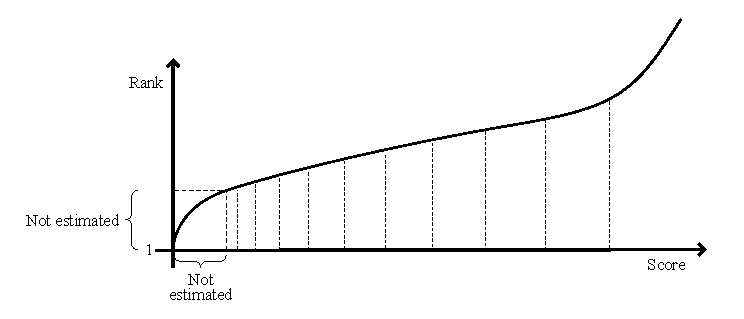
\includegraphics[width=13cm]{img/growing_bucket_sizes.eps}
\end{figure}

However, the method described above may not be enough to handle the highest ranks. One reason for that may simply be that the requirements on the algorithm and ultimately the final solution do not allow approximations \emph{at all} for the top ranks. To solve that problem the approximating algorithms can be paired with the \emph{Rank by counting}-algorithm (see \cref{counting}) for the highest ranks. This should not be a problem since  the counting involves only the critical and highest ranks which can easily be fetched if the data is indexed. When to not estimate can be decided by looking at variables such as the score or rank estimate to name a few examples.


\subsection{\label{bucket}Buckets with Global Query}

An approach to ranking by doing linear interpolation is called \emph{Buckets with Global Query}\footnote{\href{https://cloud.google.com/datastore/docs/articles/fast-and-reliable-ranking-in-datastore/}{Fast and Reliable Ranking in Datastore:\\ https://cloud.google.com/datastore/docs/articles/fast-and-reliable-ranking-in-datastore/}}. A \emph{bucket} correspond to a datastructure having a \emph{start score}, \emph{rank for the start score} and the \emph{number of scores within the bucket}. A \emph{bucket-table} consists of a number of buckets. An interpolant for a score that falls into a bucket can be created with data from that bucket and the start score from the following one\footnote{Storing both lowest and highest score for a bucket would result in having to update two buckets when a new highscore would fall between the two.}

The bucket-table is created by iterating through the whole, sorted set of highscores. Table \ref{table:ranking-table} shows an example of what the table created could look like.


\begin{table}[h]
  \begin{center}
  \begin{tabular}{ c c c c }
    Bucket no & Start score & Start rank & Size \\
    5 & 1 515 & 83 & 22 \\ 
    6 & 1 961 & 105 & 23 \\ 
    7 & 2 204 & 128 & 23 \\ 
    8 & 2 574 & 151 & 24 \\  
    9 & 2 852 & 175 & 25 \\ 
  \end{tabular} 
  \caption{Excerpt from a \emph{bucket-table}}
  \label{table:ranking-table}
  \end{center} 
\end{table}

\newpage
So, for example, to approximate the rank for score $2\;050$ which falls in bucket 6, start by calculating what the score range in bucket 6 is, in this case $2\;204 - 1\;961 = 243$. $2\;050$ is $89$ scorepoints ``in'' the bucket and hence the rank is calculated as $83 + 23 \times \frac{89}{243} \approx 91$. The approximation is illustrated in Figure \ref{fig:linear}.


\begin{figure}[h!]
  \centering
  \caption{Linear interpolation}
  \label{fig:linear}
  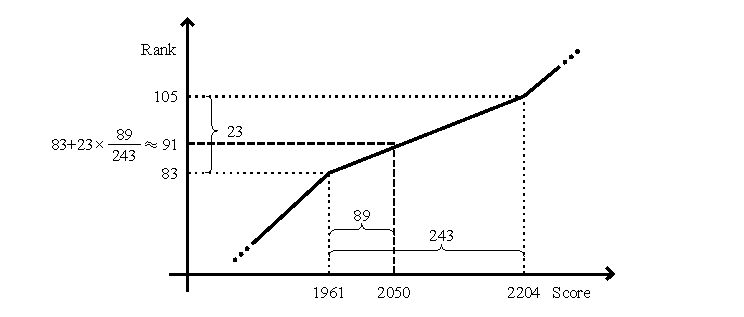
\includegraphics[width=13cm]{img/linear_interpolation.eps}
\end{figure}

\subsubsection{Quality of approximations and the lifetime of a bucket-table}

The quality of the approximations made by this method depends on several factors.
\textbf{The frequency of the periodic scans} needs to be high enough to keep the errors at an acceptable level. Also, \textbf{the size of the buckets} have an impact on the result. Yet another factor that cannot be handled in a simple way is when the score \textbf{distribution within a bucket is skewed} or not uniform within the score range as in Figure \ref{fig:uneven}.

\begin{figure}[h!]
  \centering
  \caption{An example of an uneven distribution of highscores within a bucket.
    In this case, a score in the middle of the actual distribution in the beginning of bucket a would get a rank estimate based on the score range defined by start scores of bucket a and b, which in this example would result in to a higher rank than the actual.}
  \label{fig:uneven}
  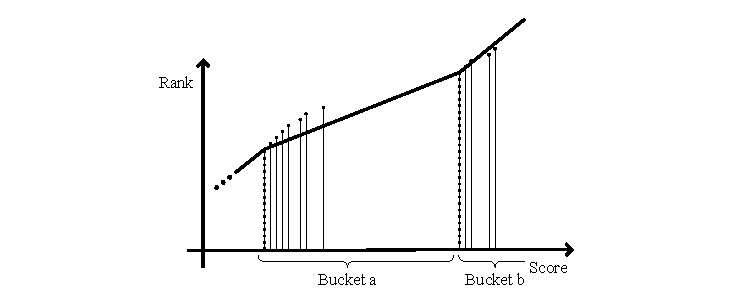
\includegraphics[width=13cm]{img/uneven_distribution.eps}
\end{figure}

When a highscore update occurs, from a lower score to a higher, but the new score falls in the same bucket as the previous highscore, the subsequent approximation will be the same as before for any score since the bucket-table is unchanged. Because the underlying highscore distribution have changed the error of the next approximation  may be different but not necessarily worse.

On the other hand, if a new highscore estimate goes from a lower rank bucket to a higher one, a subsequent scan of the highscores would result in a table where the new bucket will grow by one and, start-rank of buckets after the new bucket to and including the former one will increase by one and the bucket for the previous estimate would shrink by one.

\todo{Illustration}

% \begin{figure}[h]
%  \centering
%  \caption{A new highscore breaking the bucket-table}
%  \label{fig:change-buckets}
%  \includegraphics[width=8cm]{img/change-buckets.png}
%\end{figure}

Future highscore updates will add to the bucket-tables deviation from a theorethical \emph{true} bucket-table and as a consequence the estimates will show a growing error with respect to the true rank until the bucket-table is recreated (Figure \ref{fig:errortime}). It is worth noting that the error should not be expected to be zero even with a fresh bucket-table since approximations is precisely that -- approximations.

\begin{figure}[h]
  \centering
  \caption{Error in approximations will grow over time, until the bucket-table is recreated and the error level drops down to the initial error. Bucket-table recreated at $t_0, t_1, t_2 \dots$. 
  }
  \label{fig:errortime}
  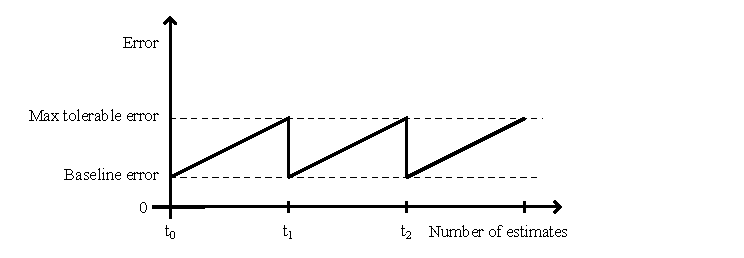
\includegraphics[width=13cm]{img/error-over-time.eps}
\end{figure}


\subsection{\label{frugal}Online approaches, streaming algorithms}

\todo{}

\iffalse

\begin{mdframed}[backgroundcolor=red,innerleftmargin=15pt,leftmargin=-10pt,rightmargin=-10pt, innerrightmargin=15pt,innertopmargin=10pt,innerbottommargin=10pt, fontcolor=white, skipabove=20pt, linewidth=0]
  
  \textbf{The rest of the chapter is not really comprehendable in its current state. I intend to finnish this section later.}
  
\end{mdframed}

The drawback with the method described above is that the bucket-table after some time will no longer represent the actual distribution of scores and consequently less and less accurate rankings.

An alternative but still similar way of solving the problem could be by estimating a number of quantiles of the distribution of highscores by using a streaming algorithm. 

\emph{Frugal streaming} is a streaming streaming algorithm for estimating a quantile of a stream devised by Ma, Muthukrishnan and Sandler. \cite{frugal_streaming} The algorithm itself is fairly self explanatory (see appendix \ref{frugal}) and have a small memory footprint.

The idea is that by calculating a number of quantiles for every new highscore while keeping track of the total number of highscores you could create a bucket-table as in the algorithm described in section \ref{bucket}.

Calculating exact quantiles of a large dataset is quite expensive.

\subsection{Quantile Digest}

\emph{Quantile Digest} is a tree based stream summary algorithm. The paper that describes the algorithm does it from a sensor network perspective 
The algorithm builds a binary tree of the value domain. The tree is then compressed and can be sent to the parent of the sensor. The compression is lossy such that less frequent values are represented as a bucket. The result of the compression is called Quantile Digest.

Quantile query - inverse quantile

\blockquote{

Inverse Quantile: Given a value x, determine its
rank in the sorted sequence of the input values.
175
In this case, we again make the same sorted list (L),
and traverse it from beginning to end. We report the
sum of counts of buckets $v$ for which $x > v.max$ as
the rank of x. The reported rank is between rank(x)
and rank(x) + $\varepsilon$, $rank(x)$ being the actual rank of
$x$.}

\fi
